\documentclass[12pt]{report}

\usepackage{geometry} % Page Dimensions
\geometry{a4paper, total={170mm,260mm}, left=20mm, top=20mm}
\usepackage{fontspec} % Γραμματοσείρες
\usepackage{xcolor} % Χρώματα
\usepackage{colortbl} % Χρωματισμός πινάκων
\usepackage{tabularx} % Πίνακες με μεταβλητό πλάτος στηλών
\usepackage{tabularray} % Πίνακες με πιο ευέλικτη διαμόρφωση
\usepackage{multicol} % Πολλαπλές στήλες (όχι για μαθηματικά)
\usepackage{hyperref} % Σύνδεσμοι στο pdf
\UseTblrLibrary{booktabs}
\usepackage{amstex} % Επιπλέον μαθηματικά εργαλεία
\usepackage{amsmath} % Μαθηματικά εργαλεία
\usepackage{amssymb}
\usepackage{tcolorbox} % Μορφοποίηση πλαισίων
\usepackage{titlesec} % Μορφοποίηση τίτλων κεφαλαίων
\usepackage{setspace} % Διάστιχο
\usepackage[greek]{babel} % Ελληνική γλώσσα
\usepackage{indentfirst} % Εσοχή πρώτης παραγράφου
\usepackage{fancyhdr} % Κεφαλίδες και υποσέλιδα
\usepackage{forest} % Δημιουργία δέντρων
\usepackage{graphicx} % Διαχείριση εικόνων
\usepackage{enumitem} % Διαμόρφωση λιστών
\usepackage{listings} % Block κώδικα
\usepackage{arabicore} %
\usepackage{booktabs} % πίνακες
\usepackage{titleps} % επικεφαλίδες και υποσέλιδα
\usepackage{lstmisc} %
\usepackage{caption}
\usepackage{tikz}

\graphicspath{ {./img/} }
%\usepackage[fontsize=13pt]{fontsize}

\setmainfont{Conduit ITC Hel Light}
\newfontfamily\fontDin{CF Din Condensed}
    \newenvironment{Din}{\fontDin}{\par}
\newfontfamily\fontDinLight{CF Din Light Condensed}
    \newenvironment{Din Light}{\fontDinLight}{\par}
\newfontfamily\fontDinMedium{CF Din Medium Condensed}
    \newenvironment{Din Medium}{\fontDinMedium}{\par}
%\newfontfamily\fontCode{Courier New}
    %\newenvironment{Code}{\fontCode}{\par}
\setmonofont[Scale=0.8]{Courier New}
\newfontfamily\fontTimes{Times New Roman}
    \newenvironment{Times}{\fontTimes}{\par}

\newfontfamily\headingfont[]{CF Din Medium Condensed}

\addto\captionsgreek{% Replace "english" with the language you use
  \renewcommand{\contentsname}%
    {ΠΕΡΙΕΧΟΜΕΝΑ}%
}

\newtcolorbox{headerdark}{colback=darkgray, boxrule=0pt,arc=0pt, boxsep=12pt,left=2pt,right=2pt,leftrule=0pt}
\newtcolorbox{headerlight}{colback=gray!50, boxrule=0pt,arc=0pt, boxsep=2pt,left=2pt,right=2pt,leftrule=0pt}
\newtcolorbox{graycomment}{colback=gray!25, boxrule=0pt,arc=0pt, boxsep=2pt,left=2pt,right=2pt,leftrule=1pt, grow to left by=-28pt,  grow to right by=-28pt}

% Το στιλ των νέων κεφαλαίων/sectionσ
\titleformat{\chapter}[block]
    {\color{black} \fontDin \large } % global formatting (number and title)
    {\color{white} \fontDin \colorbox{black!90} {\hspace{7pt}\thechapter\hspace{7pt}}} % label: number and its formatting
    {} % spacing between number and title
    {\colorbox{gray!25}} % optional (content between number and title)
\titlespacing*{\chapter}
   {0pt}{1em}{0.4em}  % left before after
\titleclass{\chapter}{straight}

\titleformat{\section}[block]
    {\color{black} \fontDinLight \large} % global formatting (number and title)
    {\color{white} \fontDin \colorbox{black!90} {\hspace{5pt}\thesection\hspace{5pt}}} % label: number and its formatting
    {} % spacing between number and title
    {\colorbox{gray!25}} % optional (content between number and title)
\titlespacing*{\section}
   {0pt}{1em}{0.4em}  % left before after

\titleformat{\subsection}[block]
    {\fontDinLight \large} % global formatting (number and title)
    {\fontDin\colorbox{gray!25} {\hspace{5pt}\thesubsection\hspace{5pt}}} % label: number and its formatting
    {\hspace{10pt}} % spacing between number and title
    {} % optional (content between number and title)
\titlespacing*{\subsection}
   {0pt}{1em}{0.4em}  % left before after

%% Setting for the column separator
%\colorlet{shadecol}{black!20}
%\setlength\columnsep{12pt}
%\makeatletter   % This change vertical bar to a dotted line
%\newcommand{\latexcolumnseprulecolor}{\color{shadecol}}
%\renewcommand\dotfill[1][0.4em]{%
%  \leavevmode\cleaders\hb@xt@ #1{\hss .\hss}\hfill\kern\z@}
%\patchcmd{\@outputdblcol}%
%  {\vrule\@width\columnseprule}%
%  {\rotatebox{90}{\parbox{\textheight}{\dotfill[0.3em]}}}%
%  {}{}
%\makeatother
%
%% Command to render shaded heading
%\newsavebox\labbox
%\NewDocumentCommand\shadedsec{O{1.5\baselineskip} O{0.33\dimexpr#1} m}{%
%  \sbox\labbox{%
%    \colorbox{black!80}{%
%      \textcolor{white}{\hspace{0.5em}#3\hspace{0.5em}}}}
%  \addvspace{#1}
%  \noindent%
%  \nopagebreak%
%  \usebox\labbox
%  {\color{shadecol}\rule[-\fboxsep]{\dimexpr\columnwidth-\wd\labbox}{\dimexpr\ht\labbox+\fboxsep}}%
%  \vspace{#2}\par}


% Ρύθμση αλλαγής γραμμής
\tolerance=1
\emergencystretch=\maxdimen
\hyphenpenalty=10000 % Για να μην κάνει συλλαβισμό στις λέξεις
\hbadness=10000

% Αλλαγή απόστασης μεταξύ παραγράφων
\setlength{\parskip}{6pt}

% Ρύθμιση Headers/Footers
\pagestyle{fancy}
\renewcommand{\headrulewidth}{0pt}
\fancyhead{}\fancyfoot{}
\fancyhead[R]{\fontDinLight ΑΛΕΞΑΝΔΡΟΣ ΞΙΑΡΧΟΣ \(\cdot\) 1059619\hspace{10pt}\colorbox{darkgray}{\color{white}\fontDin\thepage}}

% Συνεχόμενη αρίθμηση ανά chapters
\counterwithout{footnote}{chapter}

% Για γραμμές κώδικα
\lstdefinestyle{mystyle}{
    backgroundcolor=\color{gray!10},
    keywordstyle=\bf\ttfamily,
    numberstyle=\tiny\color{darkgray},
    basicstyle=\ttfamily\footnotesize,
    breakatwhitespace=false,
    breaklines=true,
    captionpos=b,
    showstringspaces=false,
    keepspaces=true,
    numbers=left,
    numbersep=5pt,
}
\lstset{style=mystyle}

\usepackage{float} % Allows for more flexible positioning of floats σε πίνακες πχ
\restylefloat{table}

% Εισαγωγή βιβλιογραφίας
\usepackage[backend=biber]{biblatex}
\addbibresource{References.bib}
\bibliographystyle{ieeetr}

\endinput

\begin{document}

    \begin{titlepage}
        \centering

        \renewcommand{\arraystretch}{1.1} % Increase row height
        \begin{tabularx}{\textwidth}{@{}m{0.9\textwidth}X@{}}
            \centering \raggedleft \cellcolor{lightgray!25} Αλέξανδρος Ξιάρχος\\ {\footnotesize st1059619@ceid.upatras.gr} & \centering\cellcolor{darkgray}\fontDin \raisebox{-1pt}{\color{white}1059619 \\}
        \end{tabularx}

        \vspace*{12em}
        \begin{headerlight}
            \begin{Din}
                \centering
                {ΠΑΝΕΠΙΣΤΗΜΙΟ ΠΑΤΡΩΝ \(\cdot\) ΤΜΗΜΑ ΜΗΧΑΝΙΚΩΝ Η/Υ ΚΑΙ ΠΛΗΡΟΦΟΡΙΚΗΣ}
            \end{Din}
        \end{headerlight}

        \begin{headerdark}
            \begin{Din Medium}
                \centering
                \huge \textcolor{white}{ΕΙΣΑΓΩΓΗ ΣΤΗ ΒΙΟΠΛΗΡΟΦΟΡΙΚΗ:\\ XML ΚΑΙ ΒΙΟΠΛΗΡΟΦΟΡΙΚΗ}
            \end{Din Medium}
        \end{headerdark}

        \begin{headerlight}
            \begin{Din}
                \centering
               ΔΕΥΤΕΡΟ ΣΥΝΟΛΟ ΑΣΚΗΣΕΩΝ \(\cdot\) 2023 \(\textendash\) 2024
            \end{Din}
        \end{headerlight}

        \vspace*{10em}

    \end{titlepage}

    \tableofcontents
    \pagebreak

%   ===================================================================================================================

    \chapter{ΕΙΣΑΓΩΓΗ}

    Η βιοπληροφορική έχει αναδειχθεί σαν ένα κομβικό επιστημονικό πεδίο ανάμεσα στη βιολογία και την επιστήμη των υπολογιστών.
    Χρησιμοποιεί υπολογιστικά εργαλεία για τη μελέτη και την κατανόηση βιολογικών δεδομένων όπως το DNA και οι πρωτεϊνες, μια διαδικασία που η ραγδαία πρόοδος των επιστημών κατέστησε απαραίτητη.
    Η βιοπληροφορική πλέον έχει εξελιχθεί σε ένα αναγκαίο εργαλείο για ερευνητικούς σκοπόυς, στην ανακάλυψη νέων φαρμάκων, στην εξατομικευμένη και προληπτική ιατρική, στη γονιδιακή θεραπεία, στη βελτιώση της καλλιέργειας κ.α.
    Η χρήση της βοηθάει στην επέκταση της γνώσης πολύ πιο αποτελεσματικά και με μεγαλύτερη ακρίβεια.

    Ο συγκεκριμένος τομέας ήρθε στο προσκήνιο με την ανακάλυψη του ανθρώπινου γονιδιώματος, κάτι που οι παραδοσιακές μέθοδοι ανάλυσης δεδομένων ήταν ανεπαρκείς για να χειριστούν τον τεράστιο όγκο των πληροφοριών που παραγόνταν.

    Μια μεγάλη πρόκληση στη βιοπληροφορική είναι η ανάγκη για τυποποίηση των τρόπων αναπαράστασης και ανταλλαγής πολύπλοκων βιολογικών δεδομένων.
    Εδώ είναι που η XML (eXtensive Markup Language) μπαίνει στο προσκήνιο.
    Πρόκειται για μια γλώσσα σήμανσης αρκετά ευέλικτη και ισχυρή για την αναπαράσταση ιεραρχικών σχέσεων (hierarchical relationships), κάτι αρκετά κοινότυπο στη μελέτη βιολογικών δεδομένων.

    Η σύνδεση μεταξύ XML και βιοπληροφορικής είναι τόσο διαδεδομένη που έχει οδηγήσει στην ανάπτυξη διάφορων ευρέως χρησιμοποιούμενων προτύπων στο τομέα που θα αναλυθούν στη συνέχεια.
    Καθώς ο τομέας της βιοπληροφορικής συνεχίζεται να εξελίσσεται, ο ρόλος των γλωσσών σήμανσης όπως η XML και των προτύπων που αυτή δημιουργεί γίνεται ολοένα και πιο σημαντικός για την ανταλλαγή και ενοποίηση δεδομένων και την παραγωγικότητα της επιστημονικής έρευνας.


% Να αναφέρω κάποιες XML υλοποιήσεις:

%The connection between XML and bioinformatics is exemplified by several widely-used data formats and standards in the field.
%    For instance, the Systems Biology Markup Language (SBML) is an XML-based format used to represent models of biological processes.
%    Similarly, the Protein Data Bank (PDB) format, which describes three-dimensional structures of proteins and nucleic acids, has an XML version called PDBML.
%    These XML-based formats enable researchers to exchange complex biological data in a structured and machine-readable manner, facilitating collaboration and data integration across different platforms and tools.
%Moreover, XML's extensibility allows for the creation of custom tags and attributes, making it possible to adapt the format to the specific needs of different subfields within bioinformatics.
%    This flexibility has led to the development of numerous XML-based standards for various aspects of biological data representation, such as MAGE-ML for microarray gene expression data, PhyloXML for phylogenetic trees, and BIOML for general biological data exchange.
    \pagebreak
    \chapter{ΑΝΑΣΚΟΠΗΣΗ ΤΩΝ ΑΡΘΡΩΝ}

\section{ΠΡΟΣΕΓΓΙΣΕΙΣ ΜΕ ΒΑΣΗ ΤΗΝ XML}
    Το άρθρο "\textit{XML-based approaches for the integration of heterogeneous bio-molecular data}" των Mesiti, Jimenez-Ruiz κ.α. πραγματεύεται κάποιες προσεγγίσεις για την αναπαράσταση, ενσωμάτωση και διαχείριση βιολογικών δεδομένων με τη χρήση γλωσσών που βασίζονται στην XML.
    Επιπλέον, παρουσιάζεται μια νέα προσέγγιση για τη διαχείριση ετερογενών βιολογικών δεδομένων μέσω της XML. \cite{XMLbasedApproaches}
    
    \subsection{Χρησιμότητα XML}
        Η XML έχει αναδειχθεί ως την πιο αποτελεσματική πρόταση για την αναπαράσταση δομημένων πληροφοριών, μιας και επιτρέπει την εύκολη επέκταση και τροποποίηση, κάτι βολικό μιας και καθημερινά δημιουργούνται και αναπτύσσονται νέα βιολογικά δεδομένα.
        Υποστηρίζεται από γλώσσες ερωτημάτων (query languages) όπως η XPath και XQuery, δίνοντας τη δυνατότητα για άμεση εξόρυξη των πληροφοριών.

        Χρησιμοποιεί μια ιεραρχική δόμηση της πληροφορίας με στοιχεία (XML Elements), χαρακτηριστικά (XML attributes) και κείμενο (XML text content).
        Κάθε στοιχείο μπορεί να αναπαριστά κάποια συγκεκριμένη βιολογική οντότητα (πχ DNA, RNA, πρωτεΐνη) και μπορεί να περιλαμβάνει εμφωλευμένα στοιχεία για συσχετιζόμενα χαρακτηριστικα.
        Αυτή η ιεραρχική δόμηση επιτρέπει την αναπαράσταση με σαφήνεια πολύπλοκων βιολογικών σχέσεων.


    \subsection{Βιολογικοί τύποι δεδομένων}
        Το άρθρο παρουσιάζει κάποιους τύπους βιολογικών δεδομένων. Για παράδειγμα:
    \begin{itemize}[label={\tiny \blacksquare}]
        \vspace{-10pt}
        \item \textbf{Δεδομένα πρωτοταγών πρωτεϊνών}: περιλαμβάνουν δεδομένα νουκλεοτιδικών αλληλουχιών, φιλοξενούνται σε βάσεις δεδομένων όπως GenBank και EMBL.
        \item \textbf{Δεδομένα πρωτεϊνών}: βάσεις δεδομένων όπως SWISSPROT και TREMBL περιέχουν πληροφορίες για πρωτεϊνικές αλληλουχίες, αναπαρίστανται εύκολα σε XML.
        \item \textbf{Motif (μοτίβα) και πρωτεϊνικές περιοχές}: προσδιορίζονται μέσω μεθόδων αναγνώρισης προτύπων που εφαρμόζονται σε δεδομένα πρωτοταγών πρωτεϊνών, αναπαρίστανται με μια περιγραφή του μοτίβου, βιβλιογραφικές πληροφορίες κ.α.
    \end{itemize}


    \subsection{Αναπαράσταση βιολογικών δεδομένων με τη χρήση XML}
        Έχουν χρησιμοποιηθεί αρκετές γλώσσες βασισμένες στην XML, ειδικά για την αναπαράσταση διαφορετικών τύπων βιολογικών δεδομένων. Για παράδειγμα:

        \subsubsection{Bioinformatic Sequence Markup Language (BSML)}
            Γλώσσα σχεδιασμένη για να περιγράφει αλληλουχίες όπως DNA, RNA και πρωτεϊνικές αλληλουχίες.
            Ένα BSML αρχείο περιλαμβάνει πληροφορίες για το πώς τα γονιδιώματα κωδικοποιούνται, ανακτώνονται και εμφανίζονται.

        \subsubsection{Protein Markup Language - ProXML}
            Χρησιμοποιείται για την αναπαράσταση πρωτεϊνικών αλληλουχιών.
            Περιλαμβάνει ένα identity section που περιέχει την περιγραφή των πρωτεϊνών και ένα data section που περιέχει ιδιότητες από αυτές τις πρωτεΐνες.

        \subsubsection{ΠΡΟΕΚΤΑΣΗ: RNA Markup Language - RNAML}
            Γλώσσα που σχεδιάστηκε με σκοπό να διευκολύνει την ανταλλαγή RNA πληροφοριών μεταξύ διαφορετικών λογισμικών βιοπληροφορικής. \cite{RNAML}
            Μέχρι πρότινος, κάθε εργαστήριο ανέπτυσσε το δικό του λογισμικό με τους δικούς του τύπους αρχείων για την ανάγνωση και την εγγραφή της βιοπληροφορίας.
            Επομένως, κατέστη αναγκαία η δημιουργία μιας τυποποίησης της RNA πληροφορίας, με σκοπό την αύξηση της αποτελεσματικότητας στην κοινότητα των βιολόγων.

            Οι προηγούμενες προσπάθειες για τυποποίηση της βιολογικής πληροφορίας περιλαμβάνουν τη γλώσσα σήμανσης BIOpolymer Markup Language (BIOML)  η οποία αναπτύχθηκε το 1999 από την ProteoMaterics.
            Περιλαμβάνει ένα framework για τον καθορισμό μοριακών οντοτήτων, και ενώ περιλάμβανε κάποιες πληροφορίες για το RNA, εστιάζονταν περισσότερο στη γονιδιακή του πλευρά
                (θέσεις έναρξης και παύσης της μεταγραφής, γενετικές τροποποιήσεις κτλ), και δεν κάλυπτε επαρκώς πληροφορίες για τη δομή του RNA, κάτι ερευνητικά κρίσιμο.
            Γενικότερα οι προηγούμενες προσπάθειες δεν κάλυπταν τις απαιτήσεις που έθετε η επιστημονική κοινότητα που μελετούσε το RNA, οδηγώντας στην ανάπτυξη της RNAML.

            Η RNAML βασίζεται πάνω στο XML.
            Υπάρχει η δυνατότητα δημιουργίας ενός Document Type Definition (DTD) το οποίο καθορίζει τη δομή του εγγράφου, τα ονόματα και τον τύπο των στοιχείων και τη ιεραρχική δομή τους,
                κάτι που διασφαλίζει τη συνέπεια και τη συμμόρφωση στο πώς αναπαρίσταται το RNA.
            Επίσης, μπορεί να αναπαριστά την αλληλεπίδραση πολλαπλών μορίων RNA, την απόσταση τους, τη σύζευξη των βάσεών τους, και οποιαδήποτε άλλη σχέση έχουν μεταξύ τους.
            Τέλος, πέρα από δυνατότητες για σχολιασμό (annotation) και documentation σε κάθε στοιχείο, είναι δυνατή η ομαδοποίηση των εμφανίσεων του ίδιου λειτουργικού RNA σε διαφορετικούς οργανισμούς,
                κάνοντας εφικτή την αναπαράσταση ευθυγραμμίσεων και κοινών δομικών συστατικών.

        \subsubsection{ΠΡΟΕΚΤΑΣΗ: System Biology Markup Language (SBML)}
            Δημιουργήθηκε στα πλαίσια του ERATO Kitano Systems Biology Project για να διευκολύνει την ανταλλαγή μοντέλων μεταξύ διαφορετικών εργαλείων προσομοίωσης και ανάλυσης. \cite{SBML}

            Ένα SBML μοντέλο περιλαμβάνεται από το Διαμέρισμα (Compartment), έναν καθορισμένο χώρο όπου συμβαίνουν οι αντιδράσεις όπως ένα κύτταρο ή ένα οργανίδιο,
                ένα Eίδος (Species), οι χημικές οντότητες που συμμετέχουν στις αντιδράσεις όπως τα ιόντα ή τα μόρια, η Αντίδραση (Reaction), η διαδικασία σχηματισμού μεταξύ των ειδών,
                η Παράμετρος (Parameter), η οποία αναπαριστά ποσότητες με συμβολικά ονόματα τοπικά η καθολικά, οι Ορισμοί Μονάδων (Unit Definitions), για τον προσδιορισμό των μονάδων που χρησιμοποιούνται στο μοντέλο,
                και τέλος οι Κανόνες (Rules), μαθηματικές εκφράσεις που ορίζουν τις τιμές των παραμέτρων ή θέτουν περιορισμούς στο μοντέλο.

            \begin{figure}[ht] \noindent\centering
                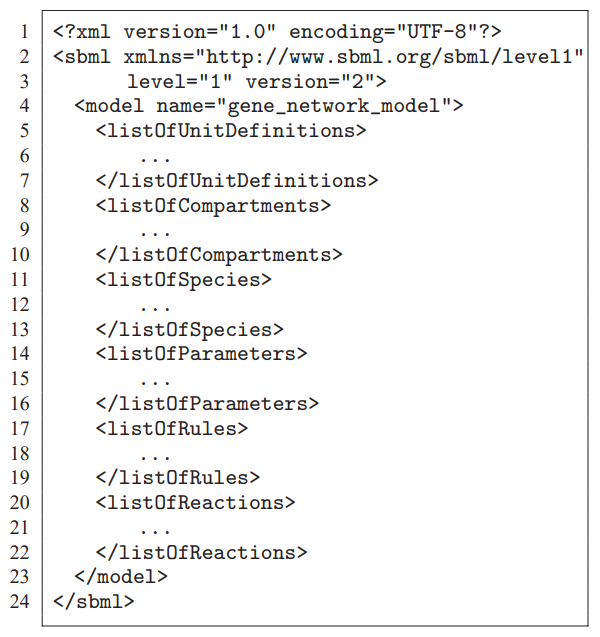
\includegraphics[scale=0.7]{img/SBML skeleton}
                \caption{Σκελετός από τον ορισμό ενός μοντέλου SBML \cite{SBML}}
            \end{figure}

        \subsubsection{ΠΡΟΕΚΤΑΣΗ: Cell Markup Language (CellML)}
            Το CellML προσφέρει μια σαφή μέθοδο ορισμού μοντέλων κυτταρικής λειτουργίας, σε ένα πιο γενικό πλαίσιο σε σχέση με τα προηγούμενα. \cite{CellML}
            Το βάθος στο οποίο μπορεί το CellML να αναπαραστήσει τις έννοιες επικαλύπτει γλώσσες όπως η SBML, με τη διαφορά ότι η SBML βασίζεται περισσότερο
                στην περιγραφή βιοχημικών αντιδράσεων, χάνοντας πληροφορία για τη δομή των μοντέλων.

            Η CellML από την αρχή σχεδιάστηκε για να υποστηρίξει μοντέλα μεγάλης κλίμακας, επιτρέπεται (λόγω της XML βάσης της) η ανεξάρτητη κατασκευή μοντέλων και τμημάτων
                και η ενσωμάτωσή τους σε ένα μεγαλύτερο μοντέλο, και παρέχει τρόπους για την απόκρυψη low-level πληροφοριών ώστε να μη συγχέονται με το υψηλότερο επίπεδο αναπαράστασης του μοντέλου.

            \begin{figure}[ht] \noindent\centering
                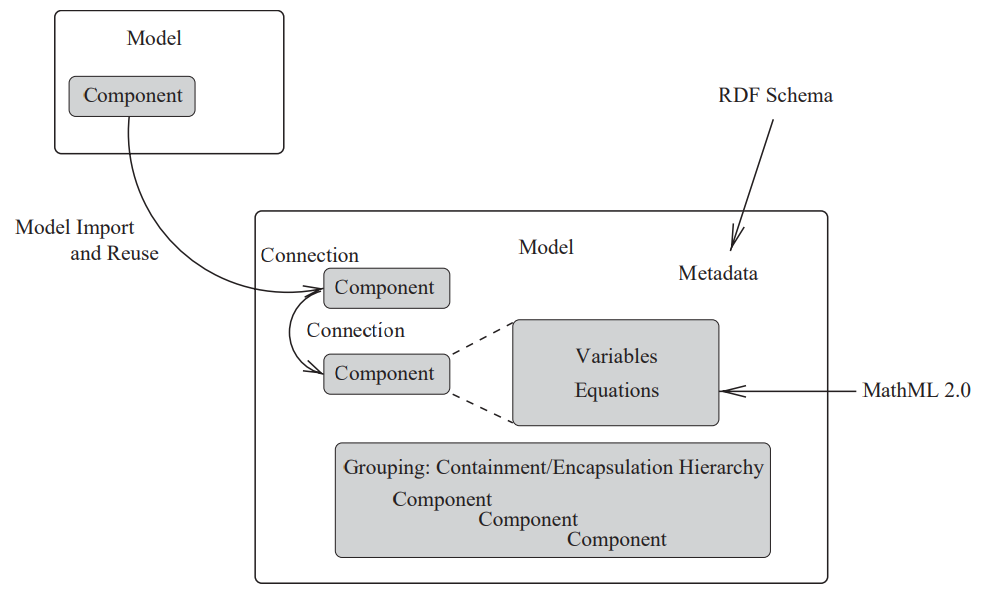
\includegraphics[scale=0.7]{img/CellML structure}
                \caption{Διάγραμμα με το σκελετό ενός CellML μοντέλου \cite{CellML}}
            \end{figure}


    \subsection{Διαχείριση ετερογενών βιολογικών δεδομένων}
        Οι βιολόγοι συνήθως χρησιμοποιούν διαφορετικές βάσεις δεδομένων, η κάθε μία με το δικό της σχεδιασμό της πληροφορίας, που καθιστά χρονοβόρα την ανάκτηση πληροφορίας.
        Επομένως, είναι αυξημένη η ανάγκη για πρόσβαση σε μια ομογενοποιημένη βάση δεδομένων, κάτι που δεν είναι πάντα εύκολο να επιτευχθεί λόγω της ετερογένειας της πληροφορίας.

        Λύση σε αυτό είναι η γλώσσα XML, που προφέρει έναν τρόπο για τη συντακτική ενσωμάτωση των δεδομένων, αν και στερείται των μεθόδων με τους οποίους μπορεί να επιτευχθεί αυτή η ενσωμάτωση.
        Τέτοιες μέθοδοι ονομάζονται αρχιτεκτονικές ενσωμάτωσης (integration architectures) και χωρίζονται στις Data warehouse, Mediator-based, Service-oriented και Peer-based αρχιτεκτονικές.

        Το δεύτερο μέρος του άρθρου αναλύει τη χρήση αυτών των αρχιτεκτονικών σε συνδυασμό με την XML για την ενσωμάτωση των δεδομένων.

        \subsubsection{ΠΡΟΕΚΤΑΣΗ: Data warehouse συστήματα}
        Η Data warehouse αρχιτεκτονική ενσωματώνει δεδομένα από διαφορετικές βάσεις δεδομένων σε μια, καταφέρνοντας μια υψηλότερου βαθμού ομογενοποίηση και χωρίς να χρειάζονται συχνές ανανεώσεις.
        Παραδείγματα τέτοιων συστημάτων είναι τα εξής:

            \paragraph{DWARF}
                Πρόκειται για ένα data warehouse σύστημα που σχεδιάστηκε για την ανάλυση μεγάλων πρωτεϊνικών οικογενειών.
                Ενσωματώνει δεδομένα που αφορούν την αλληλουχία, τη δομή και τον χαρακτηρισμό πρωτεϊνών, συνδυάζοντας δεδομένα από διαφορετικές δημόσιες βάσεις δεδομένων όπως GenBank, ExPDB, κ.α.

                Το σχεσιακό του μοντέλο δεδομένων αναπτύχθηκε στο Firebird, ένα ανοιχτού κώδικα σύστημα διαχείρισης σχεσιακών βάσεων SQL, και είναι οργανωμένο σε τρία μεγάλα τμήματα που αντιπροσωπεύουν διαφορετικές οντότητες:
                    την πρωτεΐνη (περιγράφει τη βιοχημική λειτουργία, τον οργανισμό προέλευσης και την ταξινόμηση των πρωτεϊνών), την αλληλουχία των πρωτεϊνών (σχολιασμός συγκεκριμένων θέσεων,
                        λεπτομέρειες για μεταλλάξεις) και δομή πρωτεΐνης (δεδομένα που σχετίζονται με τις δευτερογενείς και τριτογενείς δομές της πρωτεΐνης). \cite{DWARF}

            \paragraph{BioWarehouse}
                Πρόκειται για ένα toolkit ανοιχτού κώδικα που έχει σχεδιαστεί για τη διευκόλυνση της διασύνδεσης διαφορετικών βάσεων δεδομένων βιοπληροφορικής.
                Χρησιμοποιεί τη MySQL και την Oracle ως relational database managers, και επιτρέπει την ομαλή σύνδεση διαφορετικών βάσεων δεδομένων με σκοπό να γίνονται αποτελεσματικά queries και την εξόρυξη δεδομένων. \cite{BioWarehouse}

                Περιλαμβάνονται εργαλεία σε C και σε Java που κάνουν συντακτική ανάλυση (parsing) και κανονικοποιούν τα δεδομένα για να μειώσουν την ετερογένεια, ενώ έχει σχεδιαστεί ώστε να επιτρέπεται η κλιμάκωση για πολλά terabytes δεδομένων.
                Όλα αυτά κάνουν το BioWarehouse ένα χρήσιμο εργαλείο με πολλές πρακτικές εφαρμογές, όπως για παράδειγμα για τον προσδιορισμό κενών σε αλληλουχίες.

            \paragraph{Atlas}
                Data warehouse σύστημα που αποθηκεύει και ενοποιεί διαφορετικούς τύπους βιολογικών δεδομένων.
                Χρησιμοποιεί την SQL η οποία καλεί (μέσω API) εφαρμογές σε C++, Java και Perl γλώσσες, οι οποίες διαβάζουν πληροφορίες από άλλες βάσεις δεδομένων (GenBank, RefSeq, UniProt κ.α.) στη βάση δεδομένων του Atlas.
                Επίσης, περιλαμβάνει κάποια εργαλεία που χρησιμοποιούνται για την εξόρυξη δεδομένων. \cite{Atlas}

            \paragraph{Biozone}
                Ενοποιημένη πηγή για DNA αλληλουχίες, πρωτεΐνες κ.α., που ενσωματώνει μοντέλα γράφων και ιεραρχικές κλάσεις για την αναπαράσταση και την κατηγοριοποίηση βιολογικών οντοτήτων.

            \paragraph{cPath}
                Λογισμικό βάσης δεδομένων ανοιχτού κώδικα για τη συλλογή, αποθήκευση και αναζήτηση δεδομένων βιολογικών μονοπατιών.
                Τα δεδομένα μπορούν και προβάλλονται σε browser ή να εξαχθούν μέσω API που βασίζεται σε XML, κάτι που επιτρέπει τη χρήση του σε third-party εφαρμογές φτιαγμένες για την οπτικοποίηση και ανάλυση μονοπατιών.

            \begin{figure}[ht] \noindent\centering
                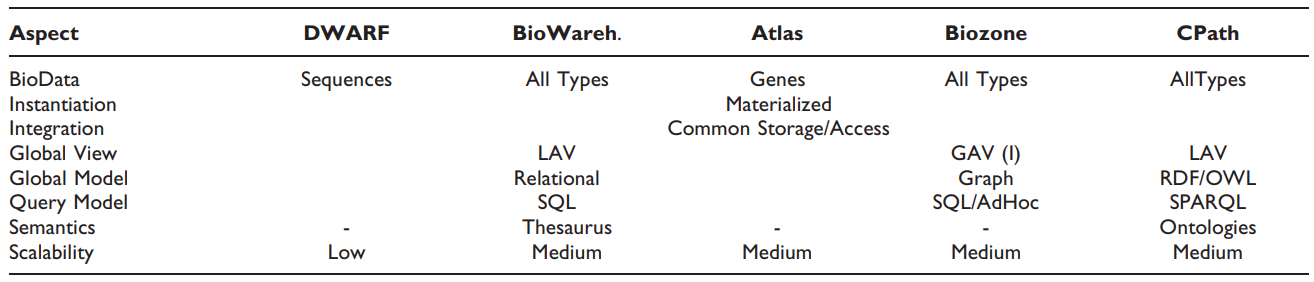
\includegraphics[scale=0.7]{img/Data warehouse table}
                \caption{Σύγκριση των Data Warehouse συστημάτων \cite{XMLbasedApproaches}}
            \end{figure}

        \subsubsection{ΠΡΟΕΚΤΑΣΗ: Mediator-based συστήματα}
            Σε αυτή την αρχιτεκτονική, οι ξένες βάσεις δεδομένων διατηρούν την αυτονομία τους και τα mediator-based συστήματα δρουν ως μεσάζοντες.
            Ο στόχος είναι η δημιουργία μιας ενοποιημένης προβολής των δεδομένων (global view) χωρίς να είναι απαραίτητη η φυσική μεταφορά των δεδομένων σε μια βάση.
            Κάθε ξεχωριστή βάση απαιτεί τον ορισμό ενός wrapper, ο οποίος θα μετατρέψει τη μορφή των δεδομένων τους (από/σε XML για παράδειγμα).

            Τα κύρια πλεονεκτήματα της συγκεκριμένης αρχιτεκτονικής είναι ότι τα δεδομένα είναι πάντα ανανεωμένα (up-to-date), δεν υπάρχουν διπλότυπα και είναι ευκολότερη η ενσωμάτωση νέων πηγών δεδομένων.

            Το μεγάλο μειονέκτημα προφανώς είναι το χειροκίνητο configuration του wrapper που απαιτείται για την ενσωμάτωση των δεδομένων, αν και έχουν προταθεί κάποιες τεχνικές αυτοματοποίησης.

            Παραδείγματα τέτοιων συστημάτων είναι τα εξής:

            \paragraph{Ontofusion}
                Σύστημα οντολογίας που βασίζεται σε δύο διεργασίες: τη χαρτογράφηση (mapping) και την ενοποίηση (unification).

                Η χαρτογράφηση είναι μια ημιαυτόματη διαδικασία που χρησιμοποιεί οντολογίες (virtual schemas) για τη σύνδεση των εξωτερικών βάσεων δεδομένων.
                Χρησιμοποιούνται τρεις μέθοδοι για τη δημιουργία των οντολογιών: η top-down (χρησιμοποιώντας μια υπάρχουσα UML οντολογία), η bottom-up (χτίζοντας μια νέα οντολογία) και ο συνδυασμός αυτών των δύο.

                Οι οντολογίες αυτές συνενώνονται σε ένα ξεχωριστό <<global schema>> όπου πλέον είναι ομογενοποιημένες.  \cite{Ontofusion}

            \paragraph{TAMBIS}
                To TAMBIS (Transparent Access to Multiple Bioinformatics Information Sources) χρησιμοποιεί την Tambis Οντολογία (TAO), ως ένα κοινό framework για την ενσωμάτωση διαφορετικών βάσεων δεδομένων.
                Υπάρχουν δύο εκδοχές του, μια unlinked εφαρμογή που επιτρέπει στον χρήστη να πλοηγηθεί σε ένα μοντέλο με 1800 βιολογικές έννοιες και ένα μοντέλο που είναι συνδεδεμένο με εξωτερικές βάσεις δεδομένων. \cite{TAMBIS}

            \begin{figure}[ht] \noindent\centering
                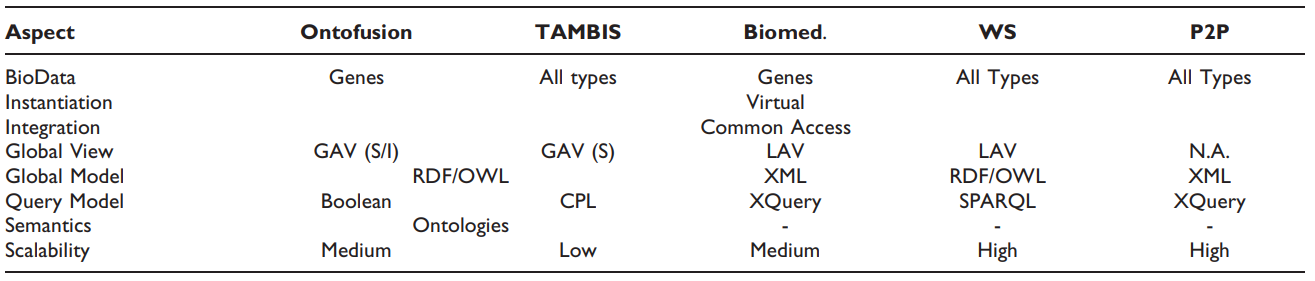
\includegraphics[scale=0.7]{img/Mediator based table}
                \caption{Σύγκριση των Mediator-based συστημάτων \cite{XMLbasedApproaches}}
            \end{figure}

        \subsubsection{Service-oriented συστήματα}
            Η Service-oriented αρχιτεκτονική προσφέρει μια τυποποιημένη μέθοδο για την ενσωμάτωση και των δεδομένων και του λογισμικού, θεωρώντας τα ως υπηρεσίες.
            Έτσι οι εφαρμογές θα τις συνδυάσουν για να υλοποιήσουν τις προβλεπόμενες εργασίες τους.

        \subsubsection{Peer-based συστήματα}
            Προσφέρουν μια αποκεντρωμένη προσέγγιση για την ενσωμάτωση δεδομένων μεταξύ διαφορετικών πηγών δεδομένων σε ένα δίκτυο.
            Η αποκέντρωση προσφέρει μεγαλύτερη ευελιξία και επεκτασιμότητα, ενώ δεν είναι απαραίτητη η δημιουργία μιας κεντρικής οντολογίας στην οποία πρέπει να μετατραπούν όλα τα δεδομένα.
            Από την άλλη, αυτά τα συστήματα δεν είναι τόσο αποδοτικά, καθώς η πολυπλοκότητα των δεδομένων είναι αυξημένη.


    \subsection{Παράμετροι για την ενοποίηση των δεδομένων}
        Κάποιες από τις παραμέτρους που επηρεάζουν την αρχιτεκτονική που θα χρησιμοποιήσουμε για την ενοποίηση των δεδομένων είναι \textbf{οι τύποι των δεδομένων} (όλα βασίζονται στο XML, αλλά διαφορετικά συστήματα ενοποίησης εστιάζουν σε διαφορετικούς τύπους δεδομένων όπως αλληλουχίες, γονιδιακές εκφράσεις κτλ),
            το \textbf{global model} (η μορφή της αναπαράστασης: relation-based (SQL), tree-based (XML), graph-based (RDF)), το \textbf{query model} (οι γλώσσες που χρησιμοποιούνται για την πρόσβαση στα δεδομένα όπως SQL, XQuery κτλ), η \textbf{επεκτασιμότητα} κ.α.

    \subsection{Εξειδικευμένα θέματα στην ενοποίηση XML δεδομένων}
        Το άρθρο κάνει αναφορά σε κάποια επιπλέον ζητήματα που αφορούν την ενοποίηση των δεδομένων που βασίζονται στο XML.

        Τίθονται θέματα που αφορούν την ασφάλεια των δεδομένων, την εξέλιξη των δεδομένων λόγω της δυναμικής φύσης τους, την αποτελεσματικότητα των ερωτήσεων (queries) που θέτουμε όπως επίσης και την έλλειψη -για την ώρα- μιας τυποποιημένης αρχιτεκτονικής που να εφαρμόζεται καθολικά.

    Σε κάθε περίπτωση, γίνεται σαφές πως το XML έχει ξεκάθαρα επιτύχει ως τη συντακτική κόλλα που συνδέει διάφορες πηγές με βιολογικά δεδομένα.
    Το αρνητικό είναι πως έχει δημιουργήσει μια μεγάλη ποικιλία διαφορετικών μορφών δεδομένων, κάτι που καθιστά δύσκολη την αποτελεσματική ενσωμάτωσή τους.

    \pagebreak
    

\section{EDAM}
    Το άρθρο "\textit{EDAM: An ontology of bioinformatics operations, types of data and identifiers, topics and formats}" των Ison, Kalas, Jonassen κ.α. πραγματεύεται την οντολογία EDAM, μια οντολογία που έχει σχεδιαστεί για την κατηγοροποίηση πράξεων και τύπων δεδομένων στην βιοπληροφορική. \cite{EDAMpaper}
    Η EDAM (EMBRACE Data and Models) είναι μια οντολογία από έννοιες που είναι διαδεδομένες στην ανάλυση βιοεπιστημονικών δεδομένων, περιλαμβάνει πράξεις (operations), τύπους δεδομένων (data types), data identifiers και data formats, όπως επίσης και συνώνυμα, συναφείς όρους, ορισμούς και άλλες πληροφορίες, όλα οργανωμένα με ιεραρχικό τρόπο. \cite{EDAMsite}

    \subsection{ΠΡΟΕΚΤΑΣΗ: Τι είναι η οντολογία;}
        Γενικά οντολογία είναι μια επίσημη αναπαράσταση γνώσης σε ένα συγκεκριμένο πεδίο.
        Ορίζει ένα σύνολο εννοιών και κανόνων όπως επίσης και τις μεταξύ τους σχέσεις σε ένα δομημένο format που μπορεί να διαβαστεί εύκολα και από της μηχανές.
        Υπάρχει ιεράρχηση στις έννοιες μέσω της δημιουργίας κλάσεων, ιδιότητες (attributes) από αυτές τις έννοιες, σχέσεις (relationships) μεταξύ τους όπως επίσης και παραδείγματα (instances) από τις έννοιες.
        Μια οντολογία αναπαρίσταται σε γλώσσες σήμανσης όπως η OWL (Web Ontology Language) ή RDF (Resource Description Framework XML), γλώσσες που έχουν βασιστεί πάνω στην XML. \cite{OntologyWiki} \cite{BioOntologies}

    \subsection{Πώς δημιουργήθηκε η ανάγκη για να δημιουργηθεί η οντολογία EDAM;}
        Σε μια εποχή ταχείας ανάπτυξης της βιολογίας και της πληροφορικής με αποτέλεσμα την αύξηση των πληροφοριακών αναγκών, μέχρι πρότινος δεν υπήρχε μια ολοκληρωμένη οντολογία με σωστές ταξινομημένες πληροφορίες κατά ένα τρόπο που να υποστηρίζονται πράξεις μεγάλης κλίμακας.
        Τα λεξικά και οι οντολογίες που είχαν δημιουργηθεί ως τότε δεν κάλυπταν πλήρως τις ανάγκες που απαιτούσε η επιστήμη της βιοπληροφορικής.

    \subsection{Τι προσφέρει η οντολογία EDAM;}
        Η οντολογία EDAM σχεδιάστηκε με γνώμονα να είναι σχετική με τις προβλεπόμενες εφαρμογές της στη βιοπληροφορική.
        Για να επιτευχθεί αυτό, μελετήθηκαν οι υπάρχουσες οντολογίες και εργαλεία (myGrid ontology (2007), εργαλεία από την EMBRACE, BioMoby Object Ontology (2001)).
        Ακολουθούνται αρχές όπως η λογική συνέπεια (να μην υπάρχουν αντιφάσεις στην οντολογία), σαφές σημασιολογικό πεδίο (είναι καθορισμένα τα όρια του τι καλύπτει) όπως επίσης και η δυνατότητα για μελλοντικές προεκτάσεις.

    \subsection{Υλοποίηση EDAM}
        Η οντολογία χρησιμοποιεί URIs (Uniform Resource Identifiers) για τη μοναδική αναπαράσταση των εννοιών της, με τη μορφή: \verb|http://e-damontology.org/<subontology>_<localId>|.

        Υπάρχουν τέσσερις διαφορετικές υποοντολογίες: \textbf{Operation} (συνάρτηση με εισόδους και εξόδους, πχ πρόβλεψη δομής RNA), \textbf{Data} (πληροφορία, πχ αλληλουχίες) και τη δική του υπακολουθία \textbf{Identifier}, \textbf{Topic} (περιγράφει κατηγορίες, πχ <<Ανάλυση αλληλουχιών>>) και \textbf{Format} (μορφές δεδομένων, πχ FASTQ).
        Έτσι, η κλάση <<Sequence record>> για παράδειγμα αναπαρίσταται ως \verb|http://edamontology.org/data_0849|. \linebreak
        Οι σχεσιακές σχέσεις και οι υπόλοιπες ιδιότητες ορίζονται με τη μορφή: \verb|http://edamontology.org/<id>|.

        \begin{figure}[h!] \noindent\centering
            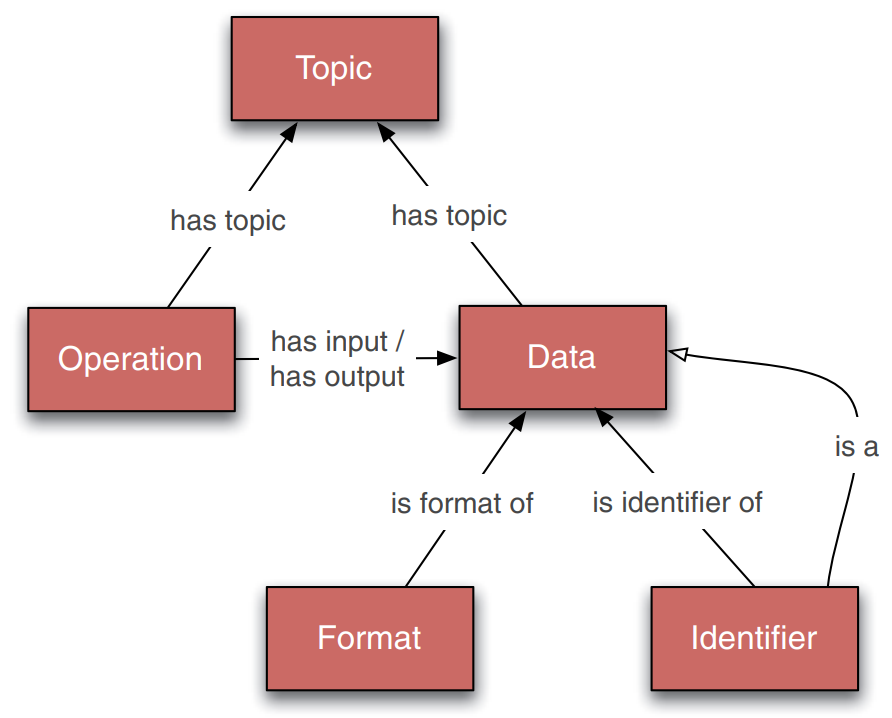
\includegraphics[scale=0.4]{img/Edam subontologies}
            \caption{Σχέσεις μεταξύ των υποοντολογιών \cite{EDAMpaper}}
        \end{figure}

% Παράγραφος 3.2
% Παραπάνω πληροφορίες για προηγούμενες οντολογίες (myGrid, BioMoby).

    \pagebreak
    \section{METATRON}
    Το άρθρο "\textit{MetaTron: advancing biomedical annotation empowering relation annotation and collaboration}" των Irrera, Marchesin κ.α. πραγματεύεται το εργαλείο MetaTron.

    Πρόκειται για μια εφαρμογή ανοιχτού κώδικα με σκοπό τη βελτίωση της αποτελεσματικότητας του σχολιασμού (annotation) βιοϊατρικών δεδομένων. \cite{MetaTron}

    \subsection{Τι είναι ο σχολιασμός (annotating);}
        Πρόκειται για την προσθήκη δομημένης πληροφορίας σε βιοϊατρικά κείμενα με σκοπό τη βελτίωσης της χρηστικότητάς τους για ερευνητικούς σκοπούς ή για κλινικές εφαρμογές.

        Συνήθως περιλαμβάνει τον εντοπισμό και την επισήμανση γονιδίων, πρωτεϊνών και άλλων οντοτήτων, τον καθορισμό σχέσεων μεταξύ τους (πώς ένα φάρμακο αλληλεπιδρά με μια ασθένεια ή πως σχετίζονται δύο γονίδια μεταξύ τους).
        Για να επιτευχθεί, χρησιμοποιούνται οντολογίες όπου βοηθούν στον σαφή καθορισμό των σχέσεων των εννοιών, μετατρέποντας τις έννοιες σε machine-readable οδηγώντας στον αυτοματισμό και στην εξόρυξη γνώσης.

        \subsubsection{ΠΡΟΕΚΤΑΣΗ: Κριτήρια (χειροκίνητου) σχολιασμού}
            Ο χειροκίνητος σχολιασμός, δηλαδή ο σχολιασμός που προέρχεται από τους ίδιους τους επιστήμονες \footnote{Ο αυτοματοποιημένος σχολιασμός είναι μια διαδικασία που στηρίζεται σε αλγορίθμους και στη μηχανική μάθηση.} είναι μια διαδικασία κουραστική και χρονοβόρα.
            Απαιτεί εξαιρετική εξειδίκευση από τους επιστήμονες ώστε να μπορέσουν να ταξινομήσουν με ακρίβεια τις οντότητες, να ελέγξουν για λάθη, κάτι το οποίο κοστίζει όλο και περισσότερο όσο αυξάνεται η πολυπλοκότητα και το μέγεθος των δεδομένων.

            Υπάρχουν πάρα πολλά κριτήρια που επιζητούνται από τα λογισμικά που χρησιμοποιούνται για χειροκίνητο σχολιασμό, που αφορούν τα τεχνικά χαρακτηριστικά τους, τη χρηστικότητά τους, κ.α.
            Παραδείγματα για τα τεχνικά χαρακτηριστικά είναι η διαθεσιμότητα του κώδικα, η ευκολία εγκατάστασης, η ποιότητα του documentation, το κόστος, ενώ για τη χρηστικότητά τους οι σημειώσεις πολλαπλών ετικετών (multi-label annotations), ενσωμάτωση με οντολογίες, προσχολιασμούς βάση προηγούμενων δεδομένων, απόρρητο δεδομένων κα.

            Έρευνα \cite{ManualAnnotating} που έγινε για τα σημαντικότερα χαρακτηριστικά, κατέληξε ότι τα σημαντικότερα είναι:
            \vspace{-10pt}
            \begin{itemize}[label={\tiny \blacksquare}]
                \item να είναι διαθέσιμο διαδικτυακά ή να μπορεί να εγκατασταθεί εύκολα
                \vspace{-7pt}
                \item να είναι λειτουργικό, με διαισθητικές λειτουργίες χωρίς να απαιτεί μεγάλο επίπεδο εμπειρίας από τον χρήστη
                \vspace{-7pt}
                \item να υποστηρίζει σχηματική αναπαράσταση με ευέλικτα εργαλεία που να καλύπτουν πολλά διαφορετικά use-cases
            \end{itemize}
            \vspace{-10pt}

            Τα λογισμικά σχολιασμού μέχρι τώρα (και αυτά που βασίζονται στη βιοϊατρική\footnote{MedTAG, BioQRator, ezTag, MyMiner, TeamTAT κα.}, και γενικού σκοπού\footnote{DocTag, brat, Catma, FLAT, LightTag, PDFAnno κα.}) δεν κάλυπταν όλα αυτά τα κριτήρια και χαρακτηριστικά ταυτόχρονα, με κάποια να υπερτερούν σε μερικά και να υστερούν σε άλλα.
            Επομένως, είναι σαφής η ανάγκη για έναν πιο αποτελεσματικό, λογισμικό σχολιασμού.


    \subsection{Ο ρόλος του Metatron}
        Το Metatron είναι από τα λίγα εργαλεία σχολιασμού που καταφέρνει να είναι αποτελεσματικό σε όλα τα προαναφερόμενα χαρακτηριστικά.
        Υποστηρίζει διαφορετικούς τύπους αρχείων, μπορεί να συνδεθεί με APIs από πήγες όπως PubMed για πρόσβαση σε επιπλέον πηγές, περιλαμβάνει διαφορετικούς τύπους σχολιασμού, δυνατότητες για συνεργατικό σχολιασμό, αυτόματες προτάσεις, παραμετροποίηση κα.

    \subsection{Χαρακτηριστικά του MetaTron}
        Το MetaTron υποστηρίζονται πολλαπλοί τύποι σχολιασμού, σχολιασμός σε επίπεδο εγγράφου (document-level) που περιλαμβάνουν την ανάθεση ετικετών σε ολόκληρα έγγραφα, και σε επίπεδο αναφοράς (mention-level) που εστιάζουν σε συγκεκριμένα τμήματα του κειμένου.
        Ο σχολιασμός σε επίπεδο κειμένου περιλαμβάνει σχόλια-ετικέτες (labels) και σχόλια-ισχυρισμούς (assertions), τα οποία μπορούν να συμπεριληφθούν σε RDF γραφήματα για καλύτερη αναπαράσταση.

        Υποστηρίζονται οι οντολογίες, επιτρέποντας στους χρήστες να ορίζουν εννοιών (concepts\footnote{Το MetaTron ορίζει ως έννοια ένα μεμονωμένο, αναγνωρίσιμο αντικείμενο με ξεχωριστή και ανεξάρτητη ύπαρξη.}),
            ο συνεργατικός σχολιασμός, πολλαπλοί τύποι αρχείων και μεγάλη παραμετροποίηση.
        Επιπλέον, περιλαμβάνει το AutoTron, ένα χαρακτηριστικό που προσφέρει προβλέψεις στο σύστημα για τον αυτοματοποιημένο σχολιασμό, σκοπεύοντας στην ενίσχυση της αποτελεσματικότητας των χρηστών.

        \subsubsection{Αρχιτεκτονική του MegaTron}
        Η αρχιτεκτονική του MegaTron χωρίζεται σε τρία επίπεδα, το επίπεδο δεδομένων (data layer), το επιχειρησιακό επίπεδο (business layer) και το επίπεδο παρουσίασης (presentation layer).

        Το επιχειρησιακό επίπεδο χρησιμοποιεί ένα REST API σε Django Python, δρώντας ως ο μεσολαβητής ανάμεσα στο επίπεδο παρουσίασης και επίπεδο δεδομένων.
        Το επίπεδο παρουσίασης αναπτύχθηκε χρησιμοποιώντας ReactJS, HTML/CSS/JS.

    \subsection{Υλοποίηση και αποτελέσματα}
        Το άρθρο μπαίνει σε μια λεπτομερή περιγραφή των χαρακτηριστικών και του τρόπου λειτουργίας του λογισμικού, όπως επίσης και έρευνα των χρηστών για το πόσο έμειναν ικανοποιημένοι, πράγματα που ανήκουν εκτός της σφαίρας της μελέτης μας.

    \pagebreak
    \section{ΤΕΛΕΥΤΑΙΟ PAPER}


    \pagebreak
    \printbibliography
\end{document}
